\documentclass[12pt]{article}
\usepackage{verbatim}
\usepackage[dvips]{epsfig}
\usepackage{color}
\usepackage{url}
\usepackage[colorlinks=true]{hyperref}

\begin{document}

\section*{GENESIS: Documentation}

{\bf Related Documentation:}
% start: userdocs-tag-replace-items related-do-nothing
% end: userdocs-tag-replace-items related-do-nothing

\subsection*{Source}

De Schutter E \& Bower JM (1994) An active membrane model of the cerebellar Purkinje cell I. Simulation of current clamp in slice. {\it Journal of Nerurophysiology}. {\bf 71}: 375--400. \\

\subsection*{Delayed Rectifier (Kdr) and Persistent Potassium Current (Km)}

\begin{figure}[h]
\centering
   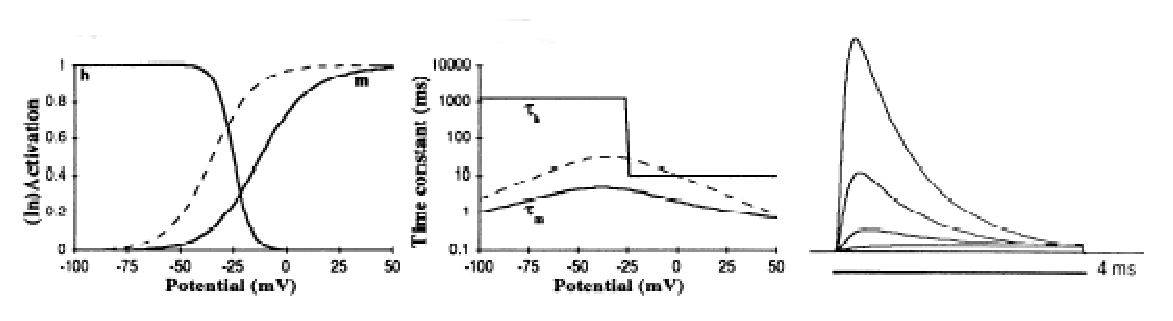
\includegraphics[scale=0.75]{figures/DS1.2E.eps}
   \caption{Activation and inactivation properties of the delayed rectifier current (Kdr, ---) and persistent K$^+$ current (Km, - - -, no inactivation) in the model. Seady-state activation and inactivation vs. voltage are plotted at the {\em left}, the time constants of activation and inactivation($\tau_m$ and $\tau_h$) vs. voltage in the {\em middle} (Note: Semilogarithmic scale), and a simulation of representative voltage-clamp currents at the {\em right}. The voltage-clamp simulation shows Kdr only and the Km current does not inactivate.}
   \label{fig:DS1.2E}
\end{figure}

\subsection*{Delayed Rectifier (Kdr)}

The Purkinje cell delayed rectifier (Kdr) is responsible for the repolarization of somatic action potentials. Whole-cell voltage-clamp recordings (Fig. 9 in\,\cite{Hirano:1989uq}) and patch-clamp recordings (Fig. 9 in\,\cite{Gahwiler:1989fk}) of the Kdr current are available but incomplete. The $I-V$ relations of the currents in both reports are very similar. In the current model we have used the published equations for Kdr current in bullfrog sympathetic ganglion cells\,\cite{Yamada-W:1989bs} because both the $I-V$ curve and the steady-state inactivation (Fig. 2E) of the bullfrog data are comparable with the data from\,\cite{Hirano:1989uq}.

\subsection*{Persistent Potassium Current (Km)}

Noninactivating K$^+$ channels in Purkinje cells have been reported by\,\cite{Bossu:1989kl} and are also apparent in recordings from\,\cite{Hirano:1989uq}. No kinetic data were available from Purkinje cells, so we have again used the equations of\,\cite{Yamada-W:1989bs} for the noninactivating muscarinic K$^+$ channel (Km).

\bibliographystyle{plain}
\bibliography{../tex/bib/g3-refs}


\end{document}
